%%%%%%%%%%%%%%%%%%%%%%%%%%%%%%%%%%%%%%
% LaTeX poster template
% Created by Nathaniel Johnston
% August 2009
% http://www.nathanieljohnston.com/2009/08/latex-poster-template/
%%%%%%%%%%%%%%%%%%%%%%%%%%%%%%%%%%%%%%

\documentclass[final]{beamer}
\usepackage[scale=1]{beamerposter}
\usepackage{graphicx}
\usepackage{listings}
\lstset{language=C++, frame=single}
\usepackage{wrapfig}
\usepackage{caption}

%-----------------------------------------------------------
% Define the column width and poster size
% To set effective sepwid, onecolwid and twocolwid values, first choose how many columns you want and how much separation you want between columns
% The separation I chose is 0.024 and I want 4 columns
% Then set onecolwid to be (1-(4+1)*0.024)/4 = 0.22
% Set twocolwid to be 2*onecolwid + sepwid = 0.464
%-----------------------------------------------------------

\newlength{\sepwid}
\newlength{\onecolwid}
\newlength{\twocolwid}
\newlength{\threecolwid}
\newlength{\fourcolwid}

%-----------------------------------------------------------
% Columns
%-----------------------------------------------------------
 %You can make columns that span multiple other columns relatively easily. Lengths are defined in the template that make columns look normal-ish if you want to use a four-column layout like this poster. If you want to use a different number of columns, you will have to modify those lengths accordingly at the top of the poster.tex file.
%        
%        In particular, near the top of the TeX file you will see lines that look like:
%        \begin{semiverbatim}
%          \hskip1ex\\setlength\{\\sepwid\}\{0.024\\paperwidth\}
%          
%          \hskip1ex\\setlength\{\\onecolwid\}\{0.22\\paperwidth\}
%          
%          \hskip1ex\\setlength\{\\twocolwid\}\{0.464\\paperwidth\}
%          
%          \hskip1ex\\setlength\{\\threecolwid\}\{0.708\\paperwidth\}
%        \end{semiverbatim}
%        
%        Set ``sepwid'' to be some small length somewhere near 0.025 (this is the space between columns). Then if $n$ is the number of columns you want, you should set
%        \begin{align*}
%          \text{onecolwid} & = \frac{1}{n}(1-(n+1)\times\text{sepwid}), \\
%          \text{twocolwid} & = 2\times\text{onecolwid} + \text{sepwid}, \\
%          \text{threecolwid} & = 3\times\text{onecolwid} + 2\times\text{sepwid}.
%        \end{align*}

\setlength{\paperwidth}{48in}            % W: 48 inches = 4 feet
\setlength{\paperheight}{36in}           % H: 36 inches = 3 feet
\setlength{\sepwid}{0.024\paperwidth}
\setlength{\onecolwid}{0.22\paperwidth}
\setlength{\twocolwid}{0.464\paperwidth}
\setlength{\threecolwid}{0.708\paperwidth}
\setlength{\fourcolwid}{0.952\paperwidth}
\setlength{\topmargin}{-0.5in}

\usetheme{confposter}
\usepackage{exscale}

%-----------------------------------------------------------
% The next part fixes a problem with figure numbering. Thanks Nishan!
% When including a figure in your poster, be sure that the commands are typed in the following order:
% \begin{figure}
% \includegraphics[...]{...}
% \caption{...}
% \end{figure}
% That is, put the \caption after the \includegraphics
%-----------------------------------------------------------

\usecaptiontemplate{
\small
\structure{\insertcaptionname~\insertcaptionnumber:}
\insertcaption}

%-----------------------------------------------------------
% Define colours (see beamerthemeconfposter.sty to change these colour definitions)
%-----------------------------------------------------------

\setbeamercolor{block title}{fg=ngreen,bg=white}
\setbeamercolor{block body}{fg=black,bg=white}
\setbeamercolor{block alerted title}{fg=white,bg=dblue!70}
\setbeamercolor{block alerted body}{fg=black,bg=dblue!10}

%-----------------------------------------------------------
% Name and authors of poster/paper/research
%-----------------------------------------------------------

\title{Open Model for Climate Behaviors}
\author{James Rising}
\institute{Ph.D. Program in Sustainable Development, Columbia
  University\\
  {\tt jar2234@columbia.edu, http://existencia.org/pro}\vspace{-1cm}}

%-----------------------------------------------------------
% Start the poster itself
%-----------------------------------------------------------

\begin{document}

\begin{frame}[fragile]

  \vspace{-4.3in}
  \hspace{2in}
  
\includegraphics[width=3in]{columbialogo.png}
 
  \vspace{-2.9in}
  \hspace{42in}
  
\includegraphics[width=3in]{../nsf1.png}

  \vspace{.3in}
  \begin{columns}[t]
   \begin{column}{1.5\sepwid}\end{column}			% empty spacer column
   \begin{column}{\onecolwid}
     \begin{block}{Motivation}
       Many of the human behaviors that drive climate change and
       environmental degradation are deeply embedded in our society,
       economy, and government, and are mutually reinforcing.  Better
       modeling of human-natural systems can help in many ways:
       \begin{itemize}
       \item Analyzing feedback loops can help identify {\bf leverage
           points}, where small policy changes can have pervasive
         impacts.
       \item Allowing models at diverse scales and contexts to
         interact can help scientists {\bf integrate knowledge}.
       \item Interactive models can facilitate {\bf communication}
         with policymakers and make complex problems intelligible.
       \end{itemize}

       \vspace{.7cm}
       The Open Model is a modeling framework aimed at these issues.  The
       boxes right describe key components.
     \end{block}
     
      \begin{block}{Applicability}
        The proposed framework provides the greatest advantage for
        problems that are currently intractable due over-determined,
        reinforcing drives, and that are spatially heterogeneous.  A
        wide range of environmental and public health issues fit this
        description, including {\bf environmental degradation,
          agricultural practices in poor countries, obesity, substance
          abuse, groundwater use, and fishery management}, as well as
        situations fraught with {\bf rebound effects} and cross-border
        shifts (e.g., {\bf carbon leakage}).

        \vspace{.5cm}
        The case studies below show some other projects that use the
        framework, in human and natural contexts.
     \end{block}

     \vspace{.3cm}
      \begin{alertblock}{Multiple Network Maps}
        Networks form the basis for models in the framework.  Models
        can play out on multiple networks simultaneously, where
        different networks can be used to describe paths upon which
        stocks flow, can divide aggregates into classes, and can
        capture the network properties of natural-human systems.
            
        \begin{figure}[h]
          {\bf Networks for Modeling Ohio}

          \vspace{.1cm}
          \fcolorbox{blue}{white}{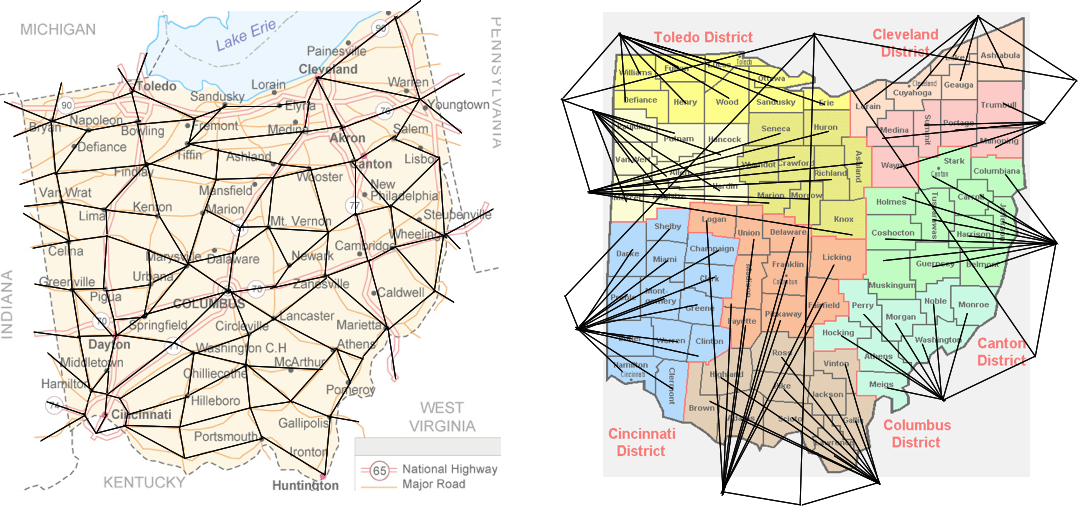
\includegraphics[width=.99\textwidth,height=3.5in]{ohionet.eps}}
          \caption*{Two rough networks for modeling Ohio
            transportation behaviors.  The left follows major roads,
            intersecting at major towns.  The right represents the
            administrative hierarchy, from counties to the state.
            Also see the hydrological case study.}
        \end{figure}
      \end{alertblock}

    \end{column}

    \begin{column}{.7\sepwid}\end{column}			% empty spacer column

    \begin{column}{\onecolwid}

      \begin{alertblock}{Overlapping Models}
        Models are inherently incomplete and different models overlap
        both conceptually and across scales.  Combining them into one
        framework and allowing them to interact both improves the
        models and allows them to specialize.  Bayesian methods are
        used to avoid runaway feedback.

        \begin{figure}[h]
          {\bf Overlapping Model Diagrams}

          \vspace{.1cm}
          \fcolorbox{blue}{white}{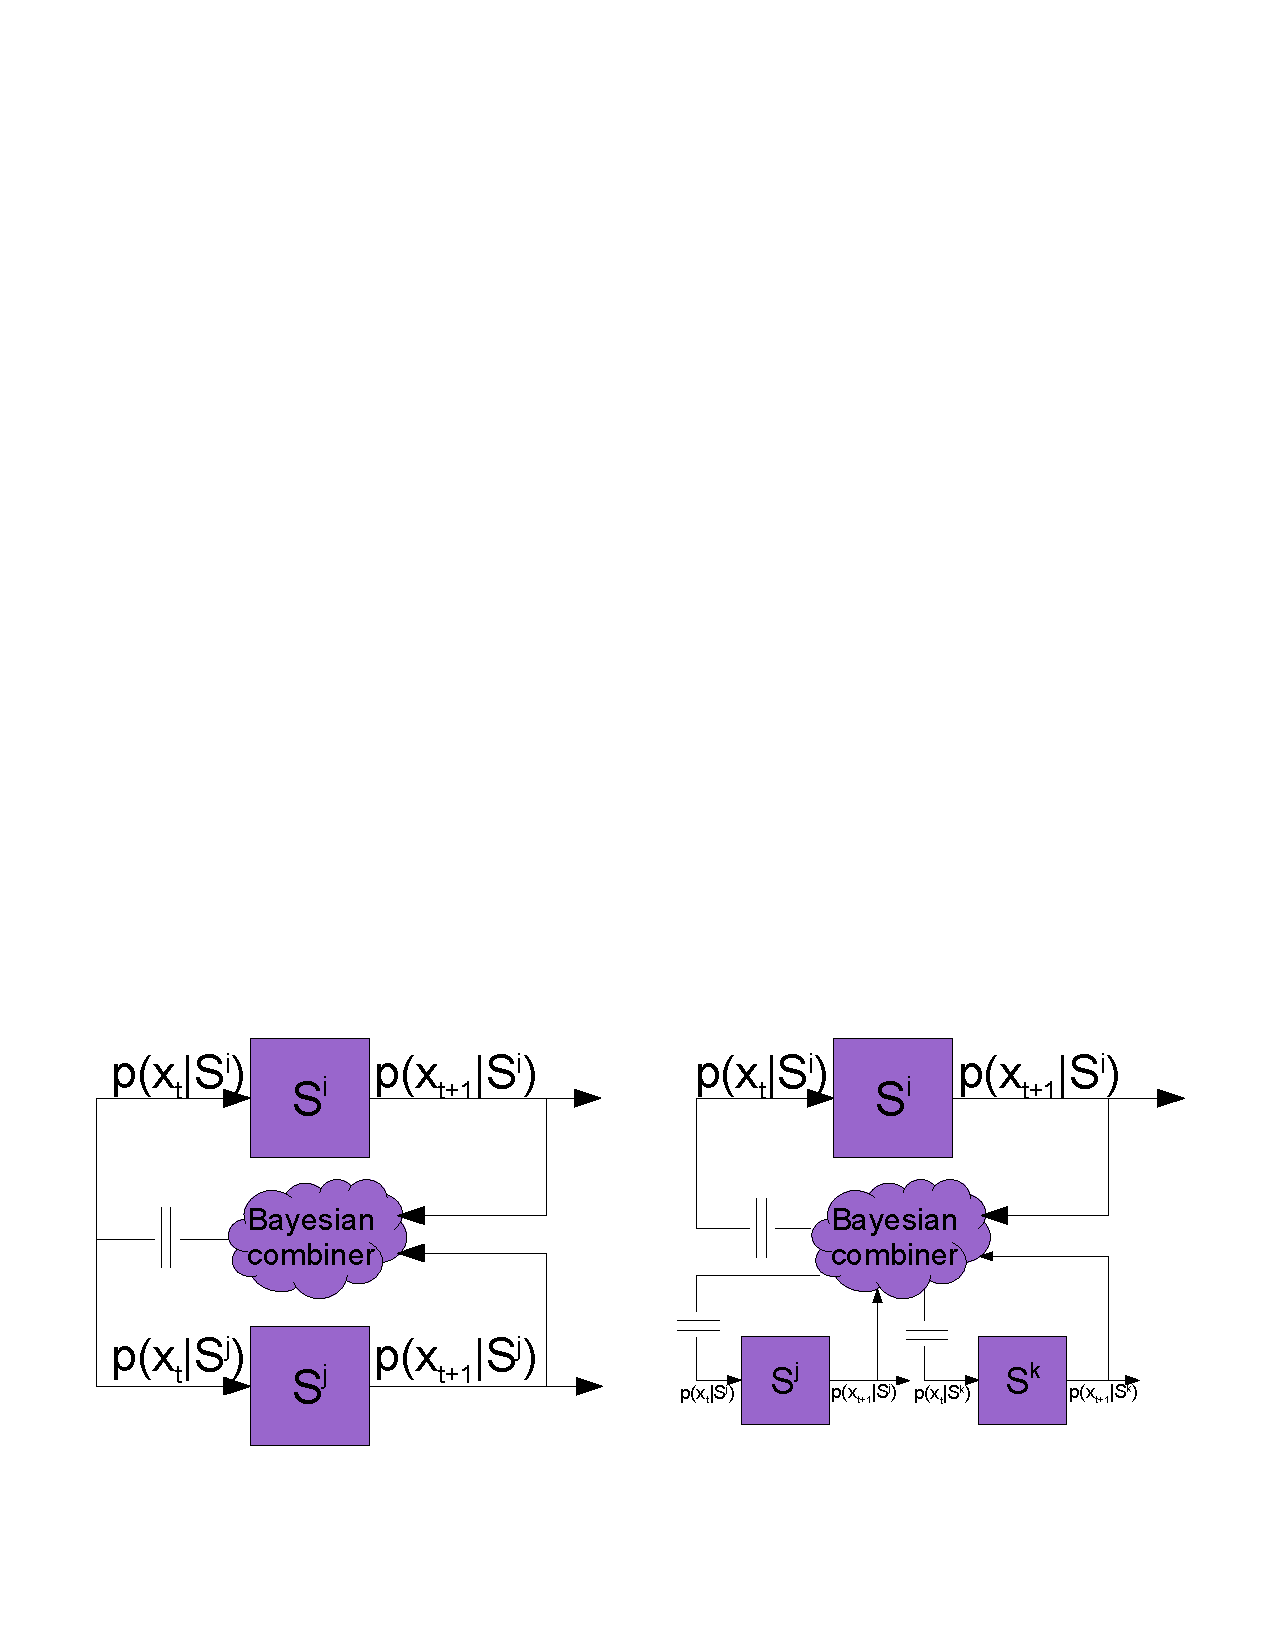
\includegraphics[width=.99\textwidth,height=3.69in]{../amalgelt.pdf}}
          \caption*{Conceptual diagrams of overlapping models.
            Left is a ``simultaneous'' model, where two models
            describe the same variable.  Right is a ``hierarchical''
            model, where an aggregate of values at one level mutually
            informs values at another level.}
        \end{figure}

        For a variable $\theta$ described by multiple models, each
        model provides both a PDF across values at a given time $t$
        when run in isolation, $p(\theta, \bar{S}^i)$, and a
        distribution that includes feedback effects, $p(\theta,
        \tilde{S}^i)$.  The final distribution is
        \[
        p(\theta | \cdot) \propto p(\theta) \prod_i p(\theta |
          \bar{S}^i)^\lambda p(\theta, \tilde{S}^i)^{1-\lambda}
        \]
      \end{alertblock}

      \begin{alertblock}{Open Interface}

        As a research platform, a transparent, open modeling framework
        provides a context for models to be evaluated, communicated,
        and learned from.

        \vspace{.5cm}
        An {\bf Website Interface} would allow researchers to explore
        the model, run tests, and contribute models.  For
        policy-makers, the online interface would provide ways to
        interact with the model, see results, and outline scenarios.

        \vspace{.5cm}
        In addition to allowing arbitrary models conforming to a
        Bayesian interface, a custom {\bf Modeling Language} combines a
        units-aware equation-like syntax with network and GIS
        features.

        \vspace{.5cm}
        \begin{figure}[h]
\begin{lstlisting}[basicstyle=\footnotesize,breaklines=true,backgroundcolor=\color{white}]
  capacity = 1e10 [tons];
  rate = 0.0077 [tons/year];
  biomass = Stock(1e7 [tons]);
  catches = TimeSeries("catches.tsv", [tons/year]);
  biomass.IncreasesBy(rate * biomass * (1 - biomass / capacity) - catches);
\end{lstlisting}
          \caption*{An example of a model written for the framework,
            for modeling fish populations.  The Networked Economics
            case study also uses this system.}
        \end{figure}

     \end{alertblock}

    \end{column}

    \begin{column}{.7\sepwid}\end{column}			% empty spacer column

    \begin{column}{\twocolwid}

      \vspace{-1.3cm}
      \begin{columns}[t]

    \begin{column}{\onecolwid}

      \begin{alertblock}{Networked System Dynamics}     
        Spatial variation matters in ecological and economic models
        and for explaining tipping points.  To help build spatially
        explicit models, relationships that drive temporal dynamics
        can be defined independently, and then applied to different
        GIS regions and networks.

        \begin{figure}[h]
          {\bf Spatial and Multi-Level Systems}

          \vspace{.1cm}
          %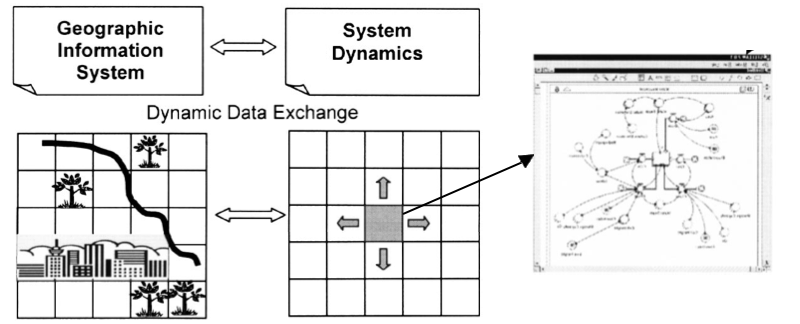
\includegraphics[width=.635\textwidth]{../opendoc/ssdarch-mod.png}
          %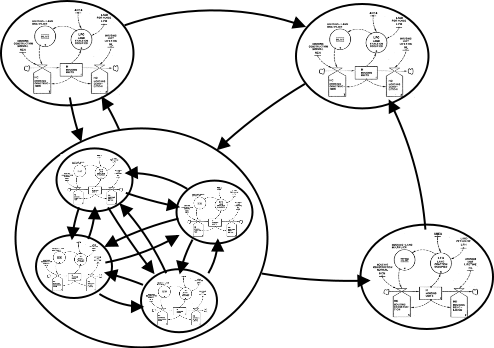
\includegraphics[width=.365\textwidth]{../opendoc/selfsimodel.png}
          \fcolorbox{blue}{white}{
            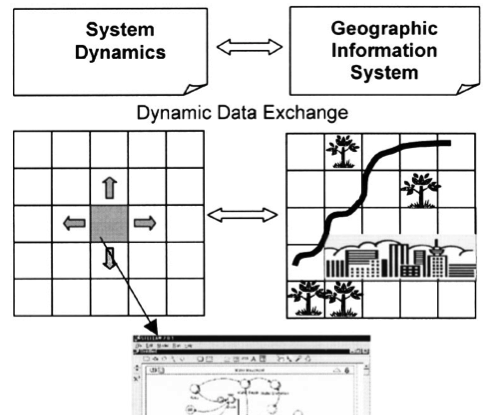
\includegraphics[width=.445\textwidth]{../opendoc/ssdarch-mod2.png}
            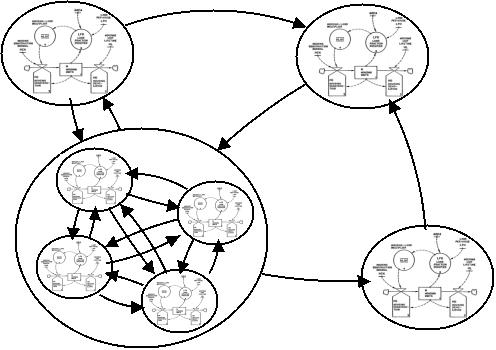
\includegraphics[width=.535\textwidth]{../opendoc/selfsimodel.jpeg}}
         \caption*{The spatial system dynamics architecture from
            \cite{ahmad2004spatial} (left) is extended into a
            networked framework (right).  Systems can be embedded
            within other systems at different spatial scales.}
        \end{figure}

        Continuing the example left of Ohio transportation, a simple
        model of networked transportation dynamics might look like
        this:

        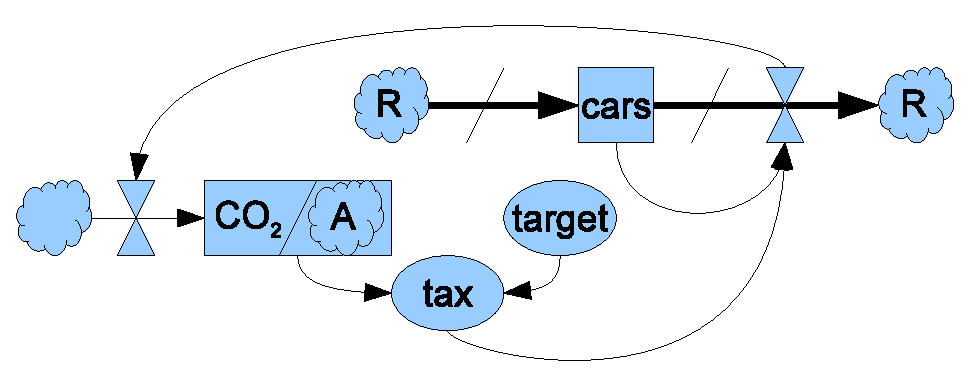
\includegraphics[width=\textwidth]{ohiomod.eps}

        Here, $\{R\}$ is the road network, upon which cars move into and
        out of a region, and $\{A\}$ is the administrative network for
        aggregating CO$_2$ contributions.

      \end{alertblock}

    \end{column}

    \begin{column}{0\sepwid}\end{column}			% empty spacer column
      
    \begin{column}{\onecolwid}
      \begin{alertblock}{Computational Tools}
        Large models can obscure the underlying causes of a system's
        behavior.  Computational tools provide ways to identify the
        important mechanisms behind different behaviors, to evaluate
        the predictive performance of models, and to construct
        simplified models for analysis and communication.

        \begin{figure}[h]
          {\bf Linear, Time-Invariant, External Error Model}
          
          \vspace{.1cm}
          \fcolorbox{blue}{white}{\includegraphics[width=.99\textwidth,height=4.28in]{../../../sysreg/syselt.png}}
          \caption*{For analysis, a simplified, linear model is
            constructed, where the time evolution of each variable is
            assumed to be composed of linear combinations of the past
            histories of other variables.  $H_{ij}$ is the
            contributing transfer function between variable $y_j(t)$
            and $y_i(t)$.}
        \end{figure}

        To determine driving feedback loops and high-leverage
        components efficiently, we construct an LTI model of transfer
        functions, informed both by data analysis (using ``system
        regressions'') and information from the models.
        \[
        \begin{pmatrix}
          y_1[t+1] \\
          y_2[t+1] \\
          \vdots \\
          y_n[t+1] \\
        \end{pmatrix}
        =
        \begin{bmatrix}
          H_{\theta_{11}}* & H_{\theta_{12}}* & \cdots &
          H_{\theta_{1n}}* \\
          H_{\theta_{21}}* & H_{\theta_{22}}* & \cdots &
          H_{\theta_{2n}}* \\
          \vdots & \vdots & \ddots & \vdots \\
          H_{\theta_{n1}}* & H_{\theta_{n2}}* & \cdots &
          H_{\theta_{nn}}* \\
        \end{bmatrix}
        \begin{pmatrix}
          y_1[t] \\
          y_2[t] \\
          \vdots \\
          y_n[t] \\
        \end{pmatrix}
        \]

        Above, $H_{\theta_{ij}} * y_j[t]$ represents the convolution
        of a discrete-time series with a transfer function.  This
        equation is analyzed in the frequency domain, where the equations
        simplify greatly.
        
      \end{alertblock}
 
    \end{column}

    \end{columns}

    \vspace{.5cm}
      \begin{block}{Climate Behavior Model Structure}
        \begin{wrapfigure}{l}{.23\textwidth}
          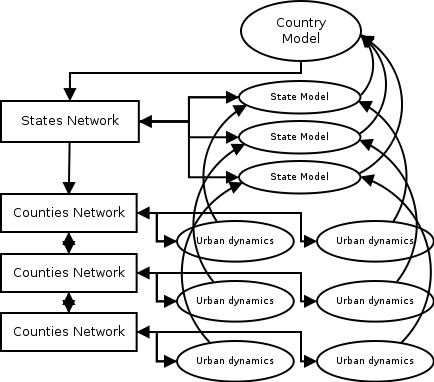
\includegraphics[width=.21\textwidth,height=3.704in]{../opendoc/architecture.png}
          \caption*{High-level structural architecture of the Open
            model for climate behaviors, described right.}
        \end{wrapfigure}

        As a first application, the Open Model will be applied to
        passenger driving behaviors.  It will include the policies,
        businesses, materials, environment, and political economy
        surrounding and influencing the actions of American drivers.
       
        \vspace{.5cm}
        To capture the multi-scale dimensions of this problems, the
        model starts with different models at a country, state, and
        urban level, connected through networks.  Aggregate dynamics
        from the Country Model (based on \cite{meadows2004limits}) are
        distributed through the States Network to each state's model
        (which is a modified version of the Country Model). The State
        Models relay stocks between each other through the States
        Network, and inform the Country Model. Each node in the State
        Network is associated with a Counties Network (that is, each
        state is divided into counties). The results of each State
        Model are further distributed to Urban dynamics models (based
        on \cite{forrester1971urban}), by way of the Counties
        Networks.

        \vspace{.5cm}
        By constructing a large model (with a minimum of 2000
        variables distributed in space), capable of modeling leverage
        points at many levels, the most effective policies can be
        identified.
    \end{block}

    \end{column}

    \begin{column}{1.5\sepwid}\end{column}			% empty spacer column

  \end{columns}


%%%%%%%%%%%%%%%%%%%%%%%%%%%%%%%%% 
%%%%%%%%%%%%%% ROW 3 %%%%%%%%%%%%%

  \begin{columns}[t]
    
    \begin{column}{1.5\sepwid}\end{column}			% empty spacer column

    \begin{column}{\onecolwid}

      \begin{block}{Case Study: Networked Economics}
        \begin{wrapfigure}{l}{.38\textwidth}
          \includegraphics[width=.35\textwidth]{../../../../groups/humeco/paper/distrib.png}
          \caption*{``Boom-bust'' cycles in a networked generalization
            of the Solow economic growth model.}
        \end{wrapfigure}

        Economic growth is anything but smooth, but cannot be easily
        modeled without heterogeneous actors.  By applying a
        traditional Solow growth model to a network of firms, a
        variety of dynamics can be demonstrated, including the
        ``boom-bust'' cycle, left.
     \end{block}

    \end{column}

    \begin{column}{.5\sepwid}\end{column}			% empty spacer column

    \begin{column}{\twocolwid}

      \begin{block}{Case Study: Hydrological Modeling}
        \begin{wrapfigure}{l}{.28\textwidth}
          \includegraphics[width=.27\textwidth]{../../../pakistan/floodposter/netmap_ext.png}
          \caption*{An efficient network map of a basin.}
        \end{wrapfigure}

        Snow and ice melt form significant contributions to river base
        flows throughout the Himalayas, but their contribution to
        seasonal and catastrophic flooding is unclear.  A physical
        hydrological model was constructed on a grid, processing
        satellite-measured inputs into stream flows and floods.
        However, fine-grained modeling is computationally intensive
        for a large basin.

        \vspace{.5cm}
        Left, the topography of a river basin is
        translated into a network for greater efficiency.  Red
        represents channel flows; blue represents flow along the
        surface into channels.
      \end{block}

    \end{column}

    \begin{column}{.7\sepwid}\end{column}			% empty spacer column

    \begin{column}{\onecolwid}

      \begin{block}{Acknowledgments}

        \begin{small}
          This project is advised by Upmanu Lall (Director of the
          Water Center) and Bruce Shaw (Lamont Doherty Earth
          Observatory), at Columbia University.

          This material is based upon work supported by the National
          Science Foundation under Grant No. 1000152207.

       \begin{thebibliography}{99}
          \bibitem{ahmad2004spatial} Ahmad et al (2004). \textit{Journal of Computing in Civil Engineering} \textbf{18}.
          \bibitem{meadows2004limits} Meadows, Randers, and Meadows (2004). \textit{The limits to growth: the 30-year update}.
          \bibitem{forrester1971urban} Forrester and Karnopp (1971). \textit{Journal of Dynamic Systems, Measurement, and Control} \textbf{93}.
          \end{thebibliography}
          \end{small}

      \end{block}

    \end{column}

    \begin{column}{1\sepwid}\end{column}			% empty spacer column

  \end{columns}

\end{frame}

\end{document}

 %%%%%%%%%%%%%%%%%%%%%%%%%%%%%%%%%
 %% Core 6

      \begin{alertblock}{Integrating Data}
       Data is essential to calibration and validation of models, but
       traditionally considered external to the operation of models.
       This framework aims for a deep integration of data, constantly
       validating and driving model behavior.

        Challenges:
        \begin{itemize}
        \item What of endogenous dynamics
        \item Data library (contextual, incomplete)
        \end{itemize}
      \end{alertblock}

            \begin{wrapfigure}{l}{.35\textwidth}
              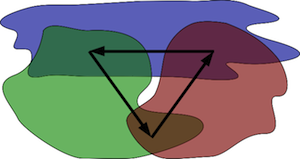
\includegraphics[width=.3\textwidth]{../blobs.png}
              \caption*{A symbolic diagram of the overlapping model system.}
            \end{wrapfigure}
            \begin{wrapfigure}{l}{.35\textwidth}
              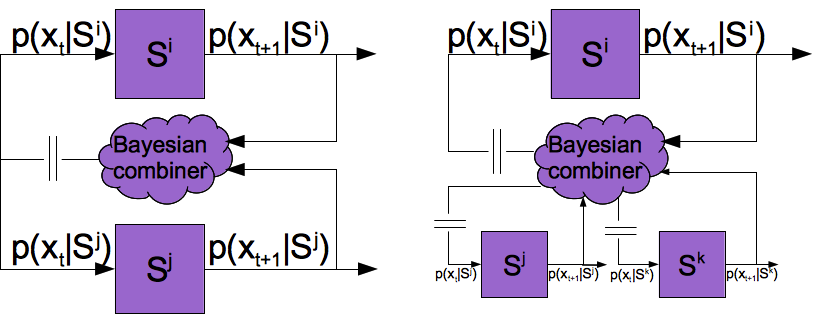
\includegraphics[width=.3\textwidth]{../amalgelt.png}
              \caption*{Element of the system regression model.}
            \end{wrapfigure}

        \begin{itemize}
        \item System regressions
        \item Driving forces simplifier
        \item Tipping/Leverage points finder
        \item Model evaluation
        \end{itemize}

        It is difficult to estimate the number of system elements
        necessary to support the search for leverage points.
        Nation-wide models range in side considerably, from 283
        variables for World3/2000 to over 2000 in the System Dynamics
        National Model.  The monumental \emph{Encyclopedia of World
          Problems and Human Potential} has identified 56,135
        ``problems,'' ranging from ``loss of cultural diversity'' to
        ``youth gangs'', and identified within them 2,675
        environmental feedback loops, ``problems that are implicated
        in many negative feedback systems concerning the natural
        environment'' \citep{ewphp}.
